\documentclass[french]{article}
\usepackage{aeguill,aecompl,babel,tikz,geometry}
\usetikzlibrary{arrows} % package de flèches
\usepackage[T1]{fontenc}
\usepackage[utf8]{inputenc}
\pagestyle{empty}
\geometry{
paperwidth=18cm,
paperheight = 7cm,
left=0pt,
right=0pt,
top=2pt,
bottom=0pt
}
%\tikzset{%
%cat/.style={right=2cm,anchor=west,align=left},
%subcat/.style={below=1cm,anchor=north west,draw=none,font=\em,align=left}
%}

%\pgfdeclarelayer{background}
%\pgfsetlayers{background,main}

\begin{document}
\centering

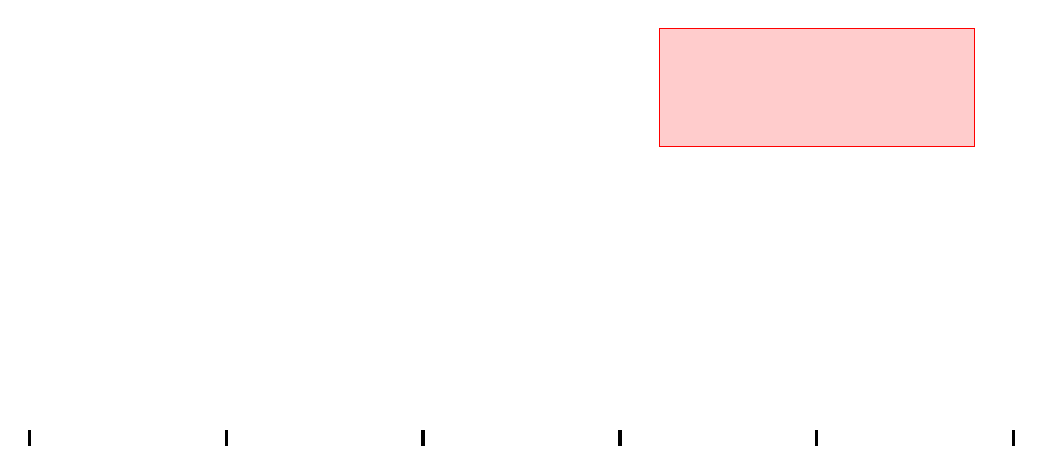
\begin{tikzpicture}
\draw [red,fill=red!20] (9,4.8) rectangle (13,6.3);
% \draw (11,5.8) node {\footnotesize{CEO}};
% \draw (11,5.3) node {\footnotesize{F Champavere}};
% \draw [red,fill=red!20] (6.8,3) rectangle (10,4.3);
% \draw (8.6,3.9) node {\footnotesize{COO}};
% \draw (8.6,3.4) node {\footnotesize{O Blanc}};
%
% \draw [blue,fill=blue!20] (4.3,1.5) rectangle (7,2.5);
% \draw (5.6,2.2) node {\footnotesize{DAF}};
% \draw (5.6,1.8) node {\footnotesize{S Zito}};
% \draw [blue,fill=blue!20] (9.8,1.5) rectangle (12.5,2.5);
% \draw (11.1,2.2) node {\footnotesize{DRH}};
% \draw (11.1,1.8) node {\footnotesize{MO Damont}};
%
% \foreach \i in {0,2.5,...,12.5}
% {\draw [gray,fill=gray!20] (\i,0) rectangle (\i+2.3,1);}
% \draw (1.1,0.7) node {\scriptsize{Dir Satisf Clt}};
% \draw (1.1,0.3) node {\scriptsize{O Blanc}};
%
% \draw (3.6,0.8) node {\scriptsize{Dir Dvlpt}};
% \draw (3.6,0.5) node {\scriptsize{grands comptes}};
% \draw (3.6,0.15) node {\scriptsize{C Barata}};
%
% \draw (6.1,0.7) node {\scriptsize{Dir BUI BUA}};
% \draw (6.1,0.3) node {\scriptsize{S Bonhomme}};
% 
% \draw (8.6,0.7) node {\scriptsize{Direction BUE}};
% \draw (8.6,0.3) node {\scriptsize{S Simon}};
%
% \draw (11.1,0.7) node {\scriptsize{Dir Log \& Qlte}};
% \draw (11.1,0.3) node {\scriptsize{D Dénizot}};
%
% \draw (13.6,0.7) node {\scriptsize{Direction BUM}};
% \draw (13.6,0.3) node {\scriptsize{D Prompt}};
% % Les lignes du diagramme
% \draw [very thick] (10.5,3.6) -- (10.5,4.8);
% \draw [very thick] (10,3.6) -- (10.5,3.6);
% \draw [very thick] (8.3,1.2) -- (8.3,3);
% \draw [very thick] (7,2) -- (9.8,2);
% \draw [very thick] (1,1.2) -- (13.5,1.2);
\foreach \i in {1,3.5,...,13.5}
{\draw [very thick] (\i,1) -- (\i,1.2);}
\end{tikzpicture}

\end{document}
